\documentclass{article}

\usepackage[margin=1in]{geometry} % Set margins to 1 inch
\usepackage{graphicx} % Allows including images
\usepackage{float} % Allows for precise placement of figures
\usepackage{amsmath} % Allows for math equations
\usepackage{siunitx} % Allows for SI units
\usepackage{placeins} % Makes sure images are in their respective sections by \FloatBarrier

\begin{document}

\title{Software Assignment Documentation\\ \large{Rayi Giri Varshini\\EE22BTECH11215}}
\author{}
\date{}
\maketitle

\maketitle

\section*{Aim}

	To make a python code which makes a playlist of songs, shuffles and allows us to play next, previous songs. The songs are shuffled in a such a way that each song of the playlist should be played atleast once and only once before it loops again.

\section*{Description}
	    Tkintker library has been used to make the window. Numpy is used to randomize the playlist. The songs should be played either by terminal or GUI(Graphical User Interphase). To play the audio files PyGame library is used. os library is used to select the directory.

\begin{figure}[ht]
	\centering
	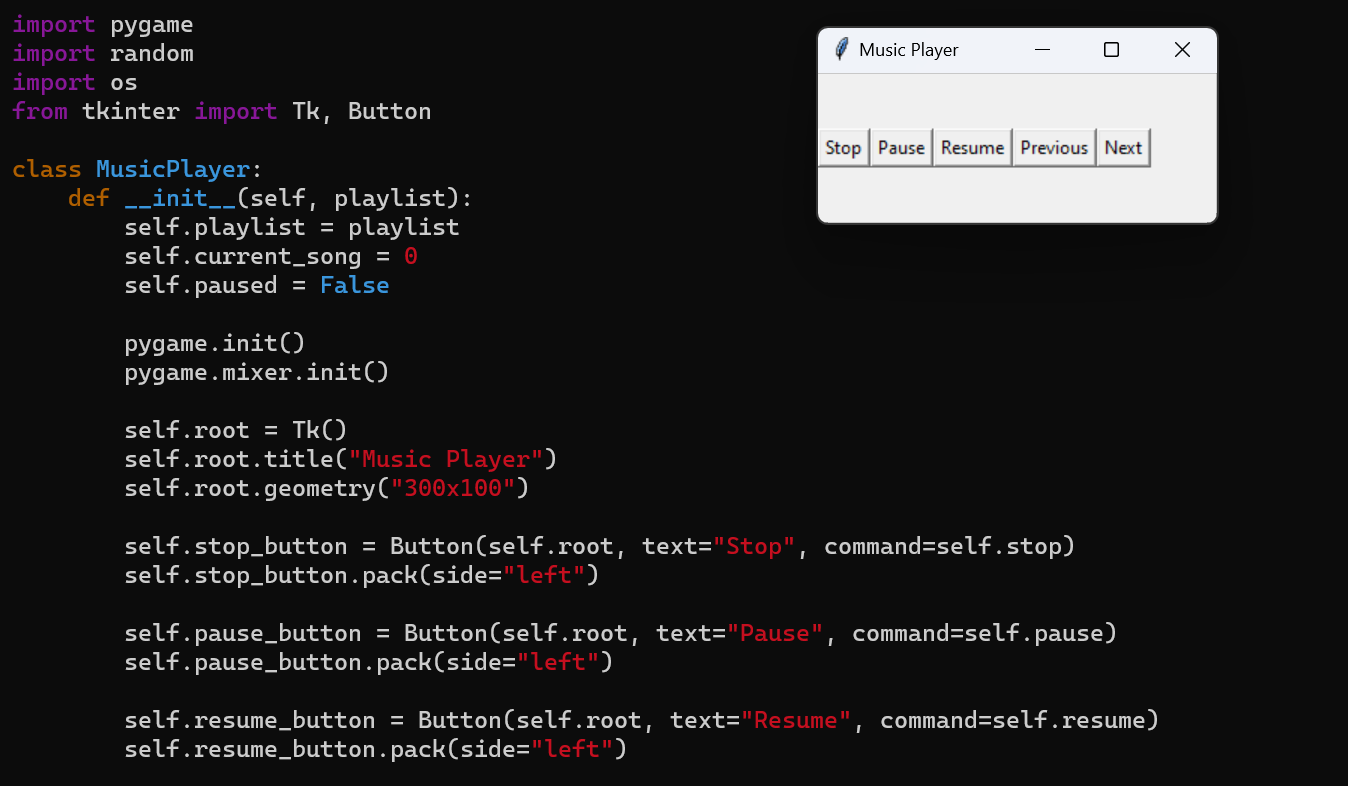
\includegraphics[width=0.7\linewidth]{software image.png}
	\caption{GUI}
	\label{fig:view}
\end{figure}
\FloatBarrier

\section*{Procedure}
     The program scans the default folder and makes a list of all the mp3 files present in it. The Shuffle function in the program randomizes the order of the audio files. As this only randomises the list, no repitition is observed. Audio file playback is handled entirely through PyGame module functions. (Pygame mixer is used).
\subsection*{Shuffle function}
\begin{enumerate}
    \item It replaces two elements with the second element to be replaced
    \item As it replaces the elements, there is no repetition in the playlist.
    \item This function is executed whenever the playlist reaches the last song and whenever the user presses next song button.
\end{enumerate}

\section*{Conclusion}

	A list of songs in a playlist can be shuffled in such a manner that they don't repeat in one loop and this runs by the users interest. The GUI makes things much easier and effiecient. The modules used for the program are pygame, tkinter, random, os.
\end{document}
